\documentclass[12pt]{extarticle}

\usepackage{wrapfig}
\usepackage{indentfirst}
\usepackage{textcomp}
\usepackage{lipsum} % Package to generate dummy text throughout this template

\usepackage[sc]{mathpazo} % Use the Palatino font
\usepackage[T1,T2A]{fontenc} % Use 8-bit encoding that has 256 glyphs
\linespread{1.05} % Line spacing - Palatino needs more space between lines
\usepackage{microtype} % Slightly tweak font spacing for aesthetics
\usepackage{amsmath,amssymb}
\usepackage[utf8]{inputenc}
\usepackage[russian,english]{babel}
\usepackage{stackengine}
\newlength\llength
\usepackage{listings}
\usepackage{color}

\usepackage[hang, small,labelfont=bf,up,textfont=it,up]{caption} % Custom captions under/above floats in tables or figures
\usepackage{graphicx}
\usepackage{subcaption}
\usepackage{booktabs} % Horizontal rules in tables
\usepackage{float} % Required for tables and figures in the multi-column environment - they need to be placed in specific locations with the [H] (e.g. \begin{table}[H])
\usepackage{hyperref} % For hyperlinks in the PDF

\usepackage{lettrine} % The lettrine is the first enlarged letter at the beginning of the text
\usepackage{paralist} % Used for the compactitem environment which makes bullet points with less space between them

\newcommand\todo[1]{\textcolor{red}{#1}}

\addto{\captionsenglish}{\renewcommand{\contentsname}{Содержание}}

\addto{\captionsenglish}{\renewcommand{\abstractname}{}}

\addto{\captionsenglish}{\renewcommand{\refname}{Список ссылок}}


\addto{\captionsenglish}{\renewcommand{\listfigurename}{Список иллюстраций}
}

\addto{\captionsenglish}{\renewcommand{\figurename}{Рис.}
}

\usepackage{pdfpages}

\begin{document}

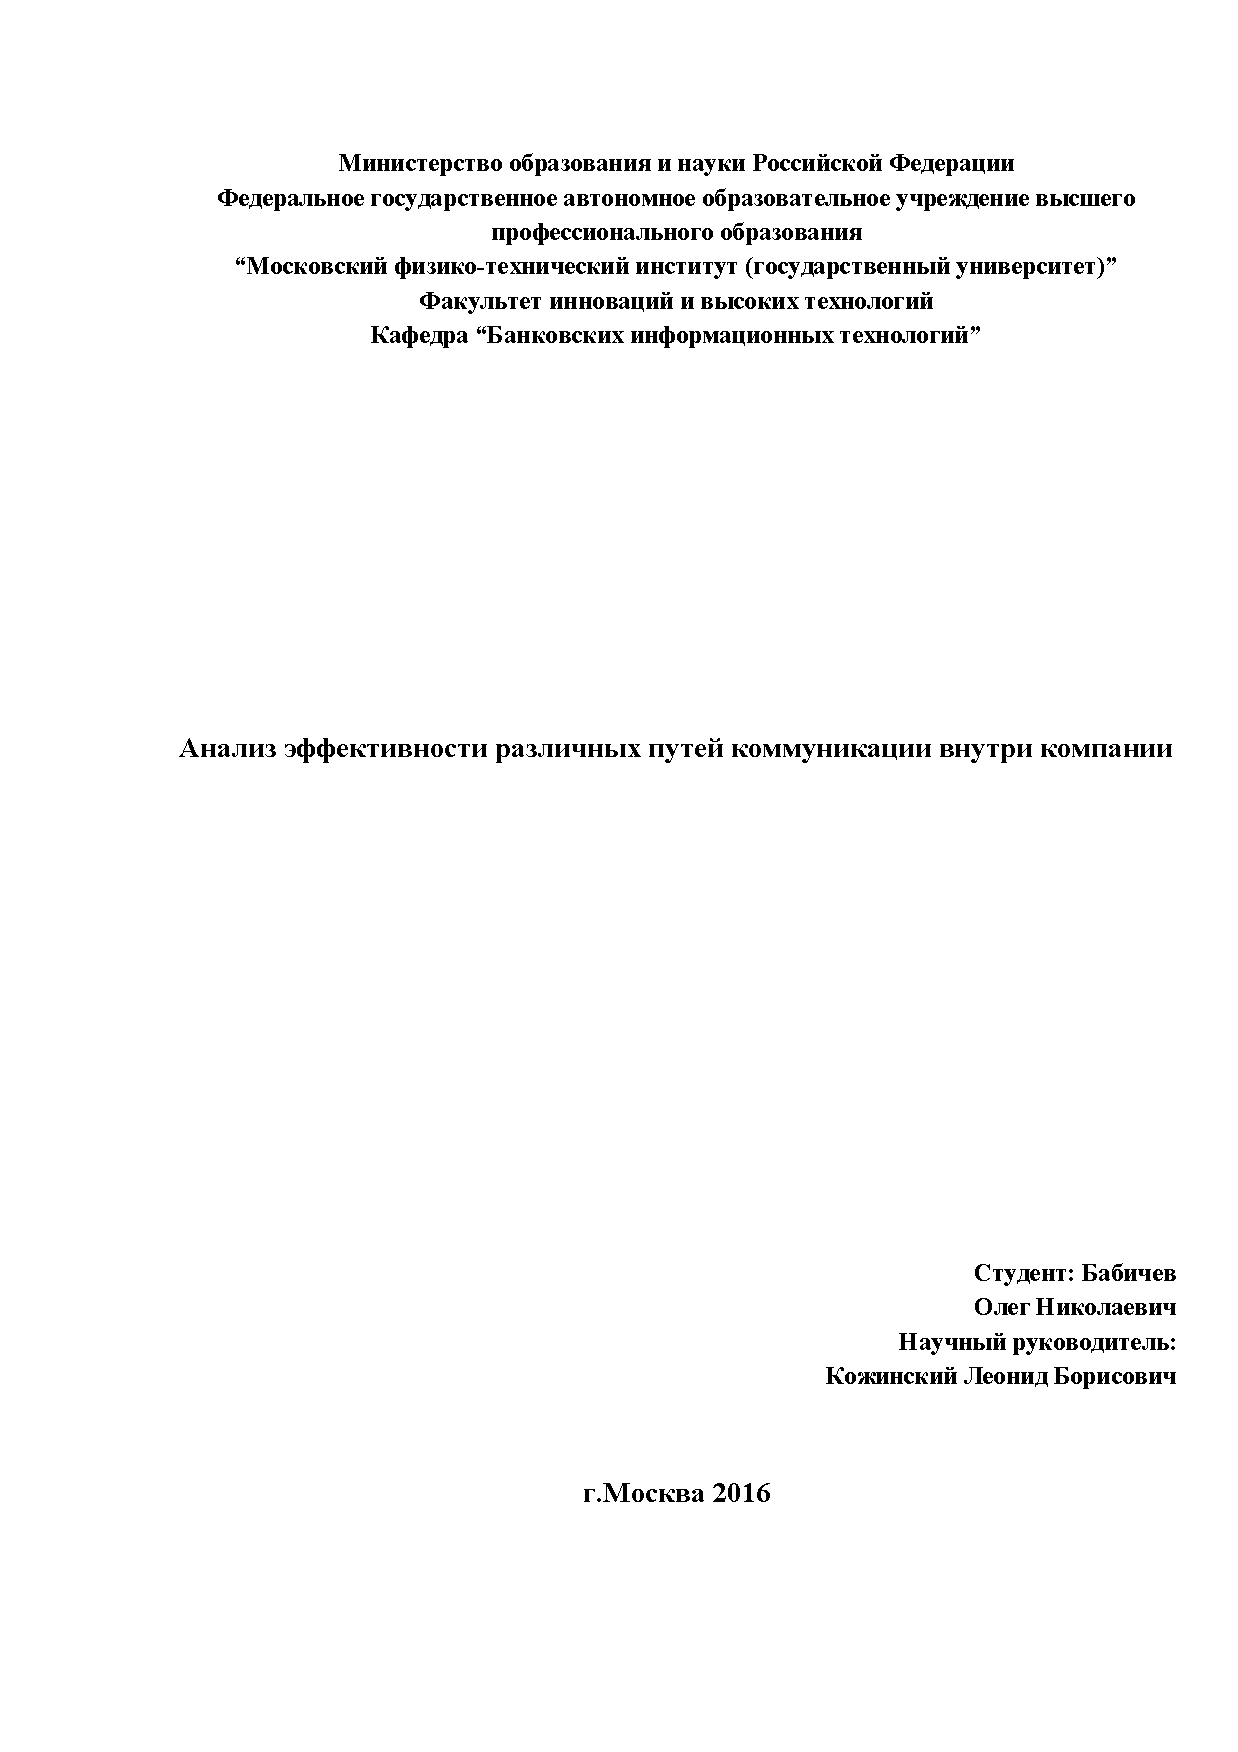
\includepdf[pages={1}]{recources/title.pdf}


\section{Введение}

Что бы вы смогли изменить в компании, если бы могли измерить вероятность того, что самые продуктивные сотрудники хотят покинуть компанию? 
Или из почтовой переписки между продавцами и покупателями определить, какой подход к клиенту приносит больше всего пользы?
В наше время по данным почтовых переписок, сообщениям в социальных сетях, историям телефонных звонков можно получить много информации о текущем положении дел в организации. 
В дальнейшем эти данные могут использоваться для улучшения результатов.

Мы работаем в организации, которая насчитывает тысячи сотрудников. Отлаженная коммуникация между этими людьми - залог успеха всей компании. 
Таким образом одна из наших задач - разработать метрики и программное обеспечение, которые позволят измерить эффективность коммуникации внутри компании. 
Исследование данных обанкротившихся компаний и открытых организаций, а также доступных внутренних почтовых переписок и телефонных звонков поможет нам выявить ключевые критерии высокой производительности компаний. 

Мы предполагаем, что изучение различных источников данных позволит выявить различные индикаторы эффективного сотрудничества. 
Эти индикаторы помогут менеджерам понять, как организовать работу группы и как ею руководить для решения той или иной задачи.

Например, исследования команды, участником которой был Питер Глур (Peter A.Gloor) \cite[p.~9]{peter_gloor_2016} показали, что творческие люди гораздо эффективнее, если у них есть строгий лидер. Хороший пример сотрудничества творческих людей - Wikipedia, в которой маленькие группы с сильным лидером создают качественные статьи быстрее, чем даже большее количество людей без лидера.

Также они выявили закономерность о том, что коллективы, в которых через определенное время меняется лидер, достигают больших результатов за то же время по сравнению с командами, в которых на протяжении всего времени работы лидер остается тем же самым.

Таким образом, изучив данные, определив метрики и выявив сами критерии, перед нами встанет задача - показать результаты непосредственно сотрудникам или командам. Питер Глур в своей статье называет "виртуальным зеркалом" ("virtual mirroring"\cite[p.~10]{peter_gloor_2016}) возвращение человеку его шаблона поведения,  возможно с какой-то оценкой или в сравнении с другими сотрудниками.

Также основываясь на многолетнем опыте Питера мы попытаемся разделить работу с каждым конкретным набором данных или конкретной организацией на 4 этапа:

\begin{enumerate}
	\item Определить метрики и шаблоны в коммуникации социальной сети. На этом этапе мы изучаем данные, выявляем шаблоны поведения и строим социальную сеть. Использую полученные данные, мы визуализируем социальную сеть и строим первоначальные гипотезы.
	\item Определить взаимосвязь между признаками социальной сети и успехами бизнеса. На этом этапе мы сравниваем результаты первого этапа с шаблонами, которые являются показателем лучшего взаимодействия внутри компании, которые нам еще предстоит выявить.
	\item Предоставить обратную связь сотрудникам или командам. Т.е. указать сотрудникам на те моменты, в которых они ведут себя не так продуктивно, как могли бы или вовсе непрофессионально. 
	\item Предоставить рекомендации по оптимизации коммуникаций для достижения еще большего успеха. Когда менеджер узнает, что именно в работе его команды нарушено и к чему именно нужно стремиться, он сможет перестроить процесс таким образом, чтобы увеличить производительность команды.
\end{enumerate}

 

\section{Степенные законы распределения}

В этой части я расскажу о функциях распределения и о том, почему мы должны обратить на них внимание. Я проделаю это на примере конкретных данных обанкротившейся компании Энрон (Enron Corporation).

Энрон - компания, достигшая большого успеха в области энергетики. Однако компания обанкротилась в 2001 году в результате бухгалтерских махинаций и сокрытия реальных доходов\cite{enron_fall}. Корпус Энрон (Enron corpus) - публичный набор данных (dataset) с историей почтовых сообщений внутри компании.

С одной стороны этот корпус может представлять большой интерес для анализа, а с другой стороны он достаточно мал (примерно полмиллиона сообщений между 158 сотрудниками\cite{sims_sinitsyn_matrix_structures}).

Функции распределения сами по себе уже давно не являются чем-то новым и необычным. Очень много вещей и величин например распределены по нормальному закону. Это происходит из следствия предельной теоремы, которое говорит о том, что если у есть множество случайных распределений, то сумма этих распределений будет похожа на нормальное распределение. 

Так распределены, например, рост человека или максимальная скорость автомобилей. Если мы говорим о распределении роста человека, то оно близко к нормальному, имеется ярко выраженный узкий пик и очень быстро затухающие хвосты. 

\todo{Можно добавить картинку с распределением роста}

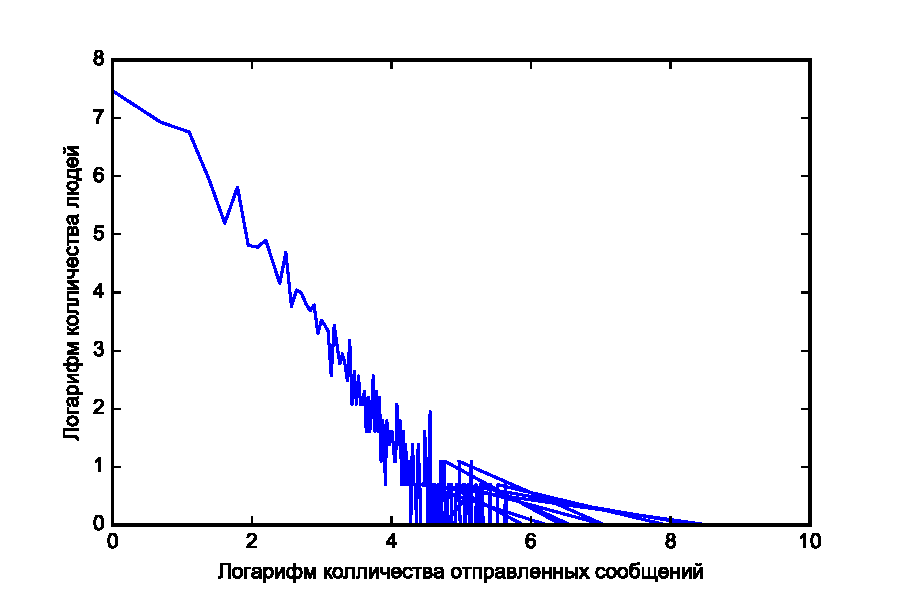
\includepdf[width=1\textwidth]{recources/mailes_by_people_enron.pdf}

Конечно же не все величины в природе распределены нормально. Есть множество исключений, например размер населения городов. В этом случае уже нет пика, функция всегда убывает. Это говорит о том, что случайно выбранный город с большей вероятностью окажется с небольшим населением и с очень низкой вероятностью огромным. 

\todo{Картинка с распределением населения городов}

Важно отметить, что встречаются города с очень большим населением, которое больше населения небольших городов на порядки, т.е. у этого распределения есть длинных хвост. И этот хвост затухает не экспоненциально, не быстро. 

Если это распределение построить в логарифмических координатах, то оно станет гораздо нагляднее и примет вид близкий к прямой. Такого вида распределения мы и будем называть \textit{степенными распределениями}. 

Это распределение имеет вид \cite{zhukov} $$ p(x) = Cx^{-\alpha} = \frac{C}{x^\alpha} \text{, для } x \ge x_{min} $$ 
Нормировка дает значение константы $C = (\alpha - 1) x_{min}^{\alpha - 1}$.
Таким образом в общем виде степенное распределение имеет вид $$p(x) = \frac{\alpha - 1}{x_{min}} \left( \frac{x}{x_{min}} \right)^{-\alpha}$$

Стоит отметить, что в этом законе распределения участвует две константы: $\alpha$ и $x_{min}$. Таким образом получается, что закон ведет семя немного по разному в зависимости от выбора начально значения. Это обусловлено тем, что нельзя определить закон из нуля.

\begin{thebibliography}{9} 

\bibitem{peter_gloor_2016} Peter A. Gloor, What Email Reveals About Your Organization. Winter 2016. 

\bibitem{zhukov} \href	{http://www.leonidzhukov.net/hse/2014/socialnetworks/lectures/lecture2.pdf}{ Power Laws. Leonid E. Zhukov. 20.01.2014.}

\bibitem{enron_fall} \href{http://www.investopedia.com/articles/stocks/09/enron-collapse.asp}{Enron: The Fall Of A Wall Street Darling. Chris Seabury}

\bibitem{sims_sinitsyn_matrix_structures} Hierarchical and Matrix Structures in a Large Organizational Email Network: Visualization and Modeling Approaches. Benjamin H. Sims, Nikolai Sinitsyn and Stephan J. Eidenbenz. Springer International Publishing Switzerland (outside the USA) 2014. DOI 10.1007/978-3-319-12188-8\_2

\end{thebibliography}

\end{document}
